% Journal of Bioinformatics and Computational Biology submission source.
% Uses the unmodified author-supplied World Scientific class dated 2026/05/18.
\pdfminorversion=7
\pdfsuppresswarningpagegroup=1
\documentclass{ws-jbcb}
\setlength{\paperheight}{11in}

\usepackage[super]{cite}
\usepackage{xcolor}
\usepackage[verbose,hypertexnames=false]{hyperref}
\hypersetup{colorlinks=false,allbordercolors=blue,pdfborderstyle={/S/U/W 1}}
\usepackage{array}
\usepackage{tabularx}
\usepackage{xurl}

\graphicspath{{./}}

% theorem, proposition, definition, example, remark, and proof are class-native.
\newtheorem{algorithm}{Algorithm}
\numberwithin{equation}{section}

\newcommand{\tas}{\textit{Arabidopsis thaliana}}
\newcommand{\ath}{\textit{A.\ thaliana}}
\newcommand{\hs}{\textit{Homo sapiens}}
\newcommand{\TAU}{\tau}
\newcommand{\xRightarrow}[1]{\stackrel{#1}{\Longrightarrow}}
\newcommand{\LTS}{\mathcal{L}}
\newcommand{\powerset}{\mathcal{P}}
\newcommand{\strongsim}{\mathrel{\sim_{s}}}
\newcommand{\weaksim}{\mathrel{\sim_{w}}}
\newcommand{\weakpre}{\mathrel{\preceq_{w}}}
\newcolumntype{Y}{>{\raggedright\arraybackslash}X}

\hypersetup{
  pdftitle={Locating resolution-dependent behavioral correspondence in qualitative DNA-damage response models},
  pdfauthor={Carlos Ramirez Ovalle},
  pdfkeywords={DNA-damage response, observational resolution, qualitative biological networks, model comparison, Petri nets, weak bisimulation}
}

\newcommand{\DRBaseMinusEdges}{5{,}062{,}632}
\newcommand{\DRBaseMinusStates}{547{,}021}
\newcommand{\DRBasePlusEdges}{10{,}296{,}917}
\newcommand{\DRBasePlusStates}{1{,}044{,}457}
\newcommand{\DRBaseSubsetBytes}{1{,}999{,}975{,}480}
\newcommand{\DRBaseSubsetPairs}{6{,}158}
\newcommand{\DRControlMinusEdges}{21{,}544{,}296}
\newcommand{\DRControlMinusStates}{2{,}140{,}569}
\newcommand{\DRControlPlusEdges}{32{,}980{,}090}
\newcommand{\DRControlPlusStates}{3{,}133{,}393}
\newcommand{\DRDepth}{8}
\newcommand{\DRDepthStates}{73}
\newcommand{\DRFirstCommitted}{1}
\newcommand{\DRHistoryStates}{78}
\newcommand{\DRLocalBaseEdges}{2}
\newcommand{\DRLocalBaseStates}{3}
\newcommand{\DRLocalMinusEdges}{54}
\newcommand{\DRLocalMinusStates}{34}
\newcommand{\DRLocalPlusEdges}{17}
\newcommand{\DRLocalPlusStates}{12}

\begin{document}

\markboth{C. Ramirez Ovalle}{Resolution-dependent behavioral correspondence}
\catchline{}{}{}{}{}

\title{Locating resolution-dependent behavioral correspondence in qualitative DNA-damage response models}

\author{Carlos Ramirez Ovalle\footnote{Corresponding author.}}

\address{Department of Natural Sciences and Mathematics, Pontificia Universidad
Javeriana Cali, Calle 18 No. 118-250, Via a Pance, Cali, Valle del Cauca,
Colombia\\
carlosovalle@javerianacali.edu.co}

\maketitle

\begin{abstract}
Models with the same stable-fate predictions can differ in whether a response
persists after a signal is withdrawn. We compare the published Calzone
death-receptor model with its documented CASP3-to-CASP8 feedback-deletion
variant, using one fixed interface observing NFkB, CASP3 and mitochondrial
permeability transition. Both variants reach survival, apoptosis and necrosis
under sustained TNF. An automatically extracted shared state follows
\DRDepth{} asynchronous updates and the visible history CASP3 activation.
From that state, sustained-stimulation continuations have the same exact
observable language. Allowing TNF withdrawal breaks correspondence: the
feedback-positive continuation preserves CASP3 and has only an apoptotic
terminal fate, whereas the feedback-negative continuation permits CASP3
deactivation and has only the model's naive terminal signature. Exact
simulation certificates and an independent model checker verify this
conditioned comparison. A verified 12-action counterexample also refutes
global sustained trace equivalence; the reverse trace inclusion remains
undecided. Thus branching alone does not separate globally trace-equivalent
biological models in this case. A secondary
DNA-damage example illustrates correspondence changes across three declared
interfaces. The study provides a reproducible relational reconstruction of a
published commitment phenomenon, not a newly discovered mechanism or wet-lab
validation.

\end{abstract}

\keywords{Cell-fate commitment; death-receptor signaling; qualitative models; signal withdrawal; weak bisimulation.}

\section{Introduction}\label{sec:introduction}

A cell-fate model may predict apoptosis during sustained stimulation without
specifying whether that response still depends on the stimulus. This distinction
matters when two mechanistic hypotheses predict the same ordinary endpoints:
the informative comparison may concern the futures remaining after an
intervention, rather than their original list of attractors. Death-receptor
signaling provides a documented setting. Calzone et al. compared a model
containing CASP3-to-CASP8 positive feedback with a variant lacking that
interaction, and analyzed the persistence of apoptosis after transient versus
sustained ligand exposure.\cite{Calzone2010} We use that published phenomenon
to ask a narrower, executable question: \emph{after a shared history and with
the same readouts, which future responses can each variant still reproduce
when TNF is withdrawn?}

Qualitative biological models make such hypotheses executable without requiring
fully parameterized kinetic descriptions.\cite{ChaouiyaPetriBio2007,Li2006,Fisher2007}
Their comparison nevertheless depends on initial conditions, update semantics,
and observable events. Structural similarity characterizes wiring, not the
availability of actions at a reachable state.\cite{Szawulak2022} Trace comparison
adds event order but can discard where alternatives cease to coexist.
Example~\ref{ex:branching} makes that mathematical distinction explicit with
early and late commitment to a choice. Here it motivates the biological
search for common observations followed by different intervention responses;
it does not predetermine that a biological pair must have equal global traces.

We apply established weak simulation and bisimulation\cite{Milner1989,Sangiorgi2011}
to finite executable models. In $X\weakpre Y$, the right-hand model must match
each step of the left-hand model and retain that ability at the resulting
state pair. Bisimulation uses one consistent relation in both directions.
The observational interface is fixed before these calculations, and hidden
internal events may be matched silently. The comparison map is
\begin{equation}\label{eq:comparison-map}
 (N_1,N_2,\Sigma)\longmapsto(\LTS(N_1),\LTS(N_2))
 \longmapsto C_\Sigma(\LTS(N_1),\LTS(N_2)),
\end{equation}
where $C_\Sigma$ reports the supported relation without assigning a biological
quality ranking to its classes.

The primary case compares the original death-receptor model, denoted DR-FB+,
with the documented feedback-deletion variant, DR-FB-. Under sustained TNF,
both have the same three reachable stable fates. We identify a shared
CASP3-positive state with exactly matching sustained continuations but different
responses to withdrawal. The full withdrawal-aware systems also have explicit
trace counterexamples in both directions. Thus the demonstrated value is an
intervention-sensitive characterization of commitment in endpoint-matched
models, not exclusive superiority over trace analysis once the discriminating
intervention is included. A verified finite counterexample also refutes global
sustained trace equivalence, so trace analysis can distinguish the complete
baseline systems as well. Only the reverse sustained trace inclusion remains
undecided; no bounded trace distance is substituted for an exact decision.

A complementary GIM (genome-instability/DNA-repair) example concerns a different
question: how correspondence changes when the interface itself changes.
Animal/human and \tas{} encodings share broad damage-response functions but
contain independently documented terminal differences.\cite{JacksonBartek2009,
BlackfordJackson2017,Yoshiyama2013,DeSchutter2007,Yi2014,Adachi2011}
Their structural similarity remains 0.9976 while correspondence is lost at the
first of three declared interfaces that exposes those differences. GIM is
retained as an illustration of interface-conditioned correspondence, not the
principal biological evidence or a search for a unique biological boundary.

The contribution is a reproducible connection between an explicit biological
perturbation question, reachable future sets, and checked relational witnesses.
It recovers an already published feedback-dependent persistence phenomenon;
neither the mechanism nor the idea of ligand withdrawal is a new discovery.
Supporting curated cases and HPN-DREAM/CASPOTS response data retain their
separate evidential roles.\cite{Hill2016,Razzaq2018}

\section{Biological comparison problem and models}
\label{sec:applications}

\subsection{Death-receptor models and the commitment question}\label{sec:death-models}

We import the original 28-node Boolean GINsim model distributed with the
Calzone study, rather than a later multiscale adaptation.\cite{Calzone2010}
DR-FB+ uses its published rules. DR-FB- changes only the CASP8 rule from
$(\mathrm{DISC\_TNF}\lor\mathrm{DISC\_FAS}\lor\mathrm{CASP3})\land
\neg\mathrm{cFLIP}$ to
$(\mathrm{DISC\_TNF}\lor\mathrm{DISC\_FAS})\land\neg\mathrm{cFLIP}$.
CASP3 remains a dynamic component; this is not its knockout.
The source article's Figures S2 and S3 explicitly examine removal of this
interaction under sustained and transient stimulation. Its previously reported
biological interpretation is therefore a rationale for the comparison, not
independent new experimental validation of our results.

The common initial state has TNF, FADD, ATP and cIAP equal to one, and all other
nodes equal to zero. FASL is zero. Each asynchronous update changes one enabled
component; FASL and FADD remain fixed. The baseline protocol also fixes TNF at
one. The intervention protocol additionally enables \texttt{withdraw\_TNF}
at every state with TNF equal to one; this action changes only TNF to zero,
irreversibly, with identical availability in both variants.

The single predeclared interface observes activation and deactivation of
NFkB, CASP3 and MPT, together with the withdrawal action. All other updates
are silent. These are the source model's survival, apoptotic and necrotic
readouts; ATP depletion is additionally required when classifying a terminal
state as necrotic. An apoptotic terminal signature has CASP3 active and
NFkB/MPT inactive; survival has only NFkB active; necrosis has only MPT active
and ATP depleted. The naive signature has all three markers inactive and ATP
present. Mixed or varying terminal signatures are reported as other, not
forced into a fate class. No such additional terminal class occurred here.

We compute reachable terminal strongly connected components and separately
check whether CASP3 can ever become inactive. A singleton reachable terminal
fate is not, in general, an inevitability claim under arbitrary scheduling.
We use \emph{model-level commitment under the declared withdrawal semantics}
for the selected state's unique apoptotic terminal fate together with
CASP3 persistence after immediate withdrawal. The selected continuation graphs
are acyclic, so their terminating post-withdrawal behavior does not require an
extra fairness assumption. This does not establish cellular commitment or
recovery from an executed biological death program.

The initial object-based enumeration exceeded 200,000 states. Before relation
results were available, we documented an unchanged-interface implementation
amendment: omit updates of the hidden sink readouts NonACD, Apoptosis and
Survival, which regulate no retained node, and enumerate retained states using
compact Boolean/CSR storage. States agreeing on all retained coordinates form
a weak bisimulation between the full model and this quotient: a sink update
stutters, while every retained update and withdrawal lifts in either direction.
All rules and initial values for the remaining components are unchanged.
Weak traces, weak relations and retained terminal signatures are preserved;
strong bisimilarity of a quotient is not automatically a strong claim about
the unreduced model. Resource amendments, source hashes and the original
configuration are retained in the reproducibility record.

\subsection{GIM as an interface-sensitivity problem}
\label{sec:gim-question}

The secondary question is whether the animal/human and \tas{} DNA-damage models
encode a common executable control organization, and at which observational
resolution that correspondence ceases to hold. Independent biology supports
comparing broad functions but also requires preserving mechanistic distinctions.
ATM- and ATR-associated sensing, checkpoint control, repair, and recovery occur
in both kingdoms; mammalian p53/apoptosis and the plant-specific SOG1, WEE1, SMR,
and damage-associated endoreduplication programs are not interchangeable
mechanisms.\cite{JacksonBartek2009,BlackfordJackson2017,Yoshiyama2013,
DeSchutter2007,Yi2014,Adachi2011,Ogita2018,ManovaGruszka2015}

We therefore evaluated three biologically motivated interfaces on exactly the
same two Petri-net structures and initial markings. Interface A observes five
coarse functions: damage detection, checkpoint activation, repair, restoration,
and exit from the proliferative cycle. Interface B additionally distinguishes
double-strand-break and replication-stress detection, ATM- and ATR-associated
signaling, and broad repair families, while retaining a common terminal
\texttt{cell\_cycle\_exit} readout. Interface C preserves those distinctions and
separately exposes mammalian \texttt{apoptosis}, plant
\texttt{smr\_induction}, and the plant net's combined
\texttt{differentiation\_or\_endoreduplication} transition. The last label is a
property of this compact encoding: the model does not infer differentiation and
endoreduplication as separate branches. Table~\ref{tab:gim-interface-rationale}
records why each process is observed or hidden. The executable definitions and
the literature keys were fixed in source data and are exported as a
machine-readable audit table.

\begin{table}[t]
\tbl{Biological rationale for the GIM observational interfaces. ``A'' denotes
coarse function; ``B/C'' denotes the pathway-resolved interfaces.
\label{tab:gim-interface-rationale}}{
\begin{tabular}{@{}>{\raggedright\arraybackslash}p{0.70in}%
>{\raggedright\arraybackslash}p{1.10in}%
>{\raggedright\arraybackslash}p{1.10in}%
>{\raggedright\arraybackslash}p{1.65in}@{}}
\toprule
Process & Animal/human encoding & \tas{} encoding & Interface treatment and
independent support \\
\colrule
Damage sensing & ATM-dominant DSB and ATR-dominant replication-stress channels
& ATM/ATR channels upstream of SOG1 & A merges detection; B/C distinguish the
initiating channels. \cite{BlackfordJackson2017,Yoshiyama2013,Adachi2011} \\
Checkpoint & CHK1/2--p53--p21 control & SOG1-regulated WEE1 and SMR
control & A exposes function; B/C expose ATM/ATR but keep downstream relays
internal. \cite{JacksonBartek2009,DeSchutter2007,Yi2014,Ogita2018} \\
Repair & DSB and excision-repair families followed by recovery & Broad
DSB and excision-repair families followed by recovery & A merges repair; B/C
separate repair families. \cite{JacksonBartek2009,ManovaGruszka2015,
Yoshiyama2013} \\
Unresolved damage & Apoptotic exit from the proliferative pool & SMR-associated
arrest followed by a combined differentiation/endoreduplication outcome & A/B
collapse terminal loss; C distinguishes encoded mechanisms.
\cite{JacksonBartek2009,Yi2014,Adachi2011,FulcherSablowski2009} \\
\botrule
\end{tabular}}
\end{table}

The interfaces are curated functional abstractions, not experimentally calibrated
observation operators. Their order was fixed for this comparison from known
mechanisms; it does not constitute a blinded prediction. The plant and animal
nets are small safe interleaving encodings, not complete DDR pathways.

\section{Computational comparison method}
\label{sec:framework}

\subsection{Labeled Petri nets and induced transition systems}
\label{sec:petri}

\begin{definition}[Labeled place/transition net]\label{def:petri-net}
A labeled place/transition net is a tuple
\begin{equation}\label{eq:petri-net}
 N=(P,T,\operatorname{pre},\operatorname{post},\ell,m_0),
\end{equation}
where $P$ and $T$ are finite sets of places and transitions,
$\operatorname{pre},\operatorname{post}:T\to\mathbb{N}^{P}$ are the input and
output multisets, $m_0\in\mathbb{N}^{P}$ is the initial marking, and
$\ell:T\to\Sigma\cup\{\TAU\}$ assigns either an observable action in the declared
interface $\Sigma$ or the internal action $\TAU$.
\end{definition}

Under standard interleaving semantics,\cite{Murata1989} $t$ is enabled at $m$ when
$\operatorname{pre}(t)\leq m$ componentwise; firing it changes $m$ to
$m-\operatorname{pre}(t)+\operatorname{post}(t)$. The implementation uses
a worklist to enumerate reachable markings explicitly. A state cap and a token
bound make failure to establish a finite state space explicit rather than silently
truncating the relation calculation. All curated Petri nets used in Section
\ref{sec:applications} are safe, but the definitions below apply to every finite
reachable system.

\begin{definition}[Finite labeled transition system]\label{def:lts}
A finite labeled transition system (LTS) is
\begin{equation}\label{eq:lts}
 L=(S,\Sigma_{\TAU},\longrightarrow,s_0),\qquad
 \Sigma_{\TAU}=\Sigma\cup\{\TAU\},
\end{equation}
where $S$ is a finite state set, $s_0\in S$, and
$\longrightarrow\;\subseteq S\times\Sigma_{\TAU}\times S$. We write
$s\xrightarrow{a}s'$ for $(s,a,s')\in\longrightarrow$. The reachable semantics
of the net in Definition \ref{def:petri-net} is denoted by $\LTS(N)$.
\end{definition}

\subsection{Observable and weak transitions}\label{sec:weak-transitions}

\begin{definition}[Silent closure and weak target sets]\label{def:weak-move}
For $s\in S$, let
\begin{equation}\label{eq:tau-closure}
 \operatorname{Cl}_{\TAU}(s)=
 \{u\in S:s\xrightarrow{\TAU *}u\}.
\end{equation}
For $a\in\Sigma$, define
\begin{equation}\label{eq:weak-target}
 W_a(s)=\{v:\exists u,w\quad
 s\xrightarrow{\TAU *}u\xrightarrow{a}w\xrightarrow{\TAU *}v\},
 \qquad W_{\TAU}(s)=\operatorname{Cl}_{\TAU}(s).
\end{equation}
We write $s\xRightarrow{a}v$ when $v\in W_a(s)$.
\end{definition}

The convention $W_{\TAU}=\operatorname{Cl}_{\TAU}$ is important: a direct silent
move on one side may be matched by zero or more silent moves on the other. It is
also the convention implemented by the Python engine and used in the AUT exports
checked by mCRL2.

\subsection{Simulation and bisimulation}\label{sec:relations}

Let $L_i=(S_i,\Sigma_{\TAU},\longrightarrow_i,s_i^0)$ for $i\in\{1,2\}$.

\begin{definition}[Weak simulation]\label{def:weak-simulation}
A relation $R\subseteq S_1\times S_2$ is a weak simulation from $L_1$ to $L_2$
if, whenever $(x,y)\in R$ and $x\xrightarrow{a}_1x'$, there is
$y'\in W_a^2(y)$ such that $(x',y')\in R$. We write
\begin{equation}\label{eq:simulation-orientation}
 L_1\weakpre L_2
\end{equation}
if $(s_1^0,s_2^0)$ belongs to some such relation. Thus the right-hand system
$L_2$ simulates the left-hand system $L_1$; the left-hand behavior is contained
in the right-hand behavior under the interface.
\end{definition}

\begin{definition}[Weak and strong bisimulation]\label{def:bisimulation}
A relation $R\subseteq S_1\times S_2$ is a weak bisimulation if it satisfies the
condition in Definition \ref{def:weak-simulation} and, for every $(x,y)\in R$ and
$y\xrightarrow{a}_2y'$, there is $x'\in W_a^1(x)$ with $(x',y')\in R$. The
initial systems are weakly bisimilar, written $L_1\weaksim L_2$, when their
initial pair belongs to such a relation. Strong bisimulation, written
$L_1\strongsim L_2$, replaces every weak target set $W_a^i(x)$ by the direct
target set $\{x':x\xrightarrow{a}_i x'\}$, including for $a=\TAU$.
\end{definition}

These are standard branching-time relations.\cite{Milner1989,Sangiorgi2011}
The explicit orientation in \eqref{eq:simulation-orientation} prevents the common
ambiguity between ``simulates'' and ``is simulated by'' in one-way results.

\subsection{Weak trace language}\label{sec:trace-language}

\begin{definition}[Exact and truncated weak traces]\label{def:weak-traces}
The finite weak observable language of $L$ is
\begin{equation}\label{eq:exact-language}
 L_w(L)=\{a_1\cdots a_r\in\Sigma^*:s_0
 \xRightarrow{a_1}\cdots\xRightarrow{a_r}s
 \text{ for some }s\in S\}.
\end{equation}
Its depth-$k$ restriction is
$L_{\leq k}(L)=\{u\in L_w(L):|u|\leq k\}$. The diagnostic distance is
\begin{equation}\label{eq:distance}
d_k(L_1,L_2)=1-
\frac{|L_{\leq k}(L_1)\cap L_{\leq k}(L_2)|}
{|L_{\leq k}(L_1)\cup L_{\leq k}(L_2)|}.
\end{equation}
\end{definition}

The implementation computes the prefix-closed truncated sets in Definition
\ref{def:weak-traces}. The statement $d_k=0$ is therefore not identified with
exact weak-trace equivalence. Exact weak-trace results come from mCRL2, acyclic path enumeration,
or finite subset-product exploration without a depth cutoff; none is inferred
from a truncated distance.

\subsection{Graded behavioral classification}\label{sec:decision}

\begin{definition}[Graded classifier]\label{def:classifier}
For finite $L_1,L_2$ over the declared interface $\Sigma$, define
$C_{\Sigma}(L_1,L_2)$ by the following priority:
\begin{equation}\label{eq:classifier}
C_{\Sigma}(L_1,L_2)=
\begin{cases}
\mathsf{strong}, & L_1\strongsim L_2,\\
\mathsf{weak}, & L_1\not\strongsim L_2\text{ and }L_1\weaksim L_2,\\
\mathsf{mutual}, & L_1\not\weaksim L_2,\ L_1\weakpre L_2,\ L_2\weakpre L_1,\\
\mathsf{left\_in\_right}, & L_1\weakpre L_2,\ L_2\not\weakpre L_1,\\
\mathsf{right\_in\_left}, & L_2\weakpre L_1,\ L_1\not\weakpre L_2,\\
\mathsf{noncomparable}, & \text{otherwise}.
\end{cases}
\end{equation}
The output is a reporting class, not a newly proposed equivalence relation.
\end{definition}

\begin{proposition}[Exclusive reporting]\label{prop:classifier}
The classifier in Definition \ref{def:classifier} assigns exactly one class to
every ordered pair of finite LTSs.
\end{proposition}

\begin{proof}
The first two cases are selected before any simulation-only case. If neither is
selected, the two simulation predicates have exactly four Boolean combinations:
both true, only the first true, only the second true, or both false. These are the
last four cases of \eqref{eq:classifier}, respectively. The cases are exhaustive
and disjoint by their stated guards.
\end{proof}

\subsection{Computational implementation}\label{sec:algorithms}

Algorithm~\ref{alg:pipeline} summarizes the executable path. Reachability and
the formal relations are exact whenever the finite state space is completed
below the declared state and token caps. The distance $d_k$, PN-GDDA, LTS-GDA,
and the structural profile are diagnostics rather than formal relations.

\begin{algorithm}[Executable comparison pipeline]\label{alg:pipeline}
\begin{romanlist}[(iv)]
\item Enumerate the reachable LTS from the initial marking or logical state by a
worklist; stop with an explicit error if a cap is exceeded.
\item Cache $\operatorname{Cl}_{\TAU}(s)$ and construct $W_a(s)$ by collecting
$a$-successors from the closure and the closures of their targets.
\item Initialize $R=S_1\times S_2$ and delete a pair immediately when it fails
the selected transfer operator; repeat complete passes until none is deleted.
\item Evaluate strong and weak bisimilarity and both simulation directions,
apply Eq.~(\ref{eq:classifier}), and attach trace and structural diagnostics.
\end{romanlist}
\end{algorithm}

The finite relation-deletion theorem and the strict hierarchy underlying
this reporting priority are proved in \ref{app:formal}.
Example~\ref{ex:branching} provides an explicit simulation witness and
a failed-successor proof for equal traces with one-way simulation.
PN-GDDA, LTS-GDA and trace distances answer complementary diagnostic
questions; their definitions and implementation checks are retained in
Supplementary Validation, Section~S1.

The accepted early/late-choice example supplies the conceptual target: equal histories need not preserve the same future choices. The biological analysis below tests a related intervention question without assuming equal global trace languages.

\section{Main result: signal withdrawal exposes a commitment difference}
\label{sec:death-results}

\subsection{Baseline agreement and its exact scope}

Complete reachable-state enumeration yields \DRBasePlusStates{} states and
\DRBaseMinusStates{} states for the two sustained-stimulation quotients.
Each has exactly three reachable singleton terminal components: survival,
apoptosis and necrosis. This is exact agreement of terminal-fate predictions,
not an assertion about matching probabilities or every transient trajectory.
An expanded exact subset-product search found a 12-action word admitted by
DR-FB+ but not DR-FB-, without changing the models or interface:
\[
\begin{split}
w={}&\mathrm{MPT}\!\uparrow,\ \mathrm{CASP3}\!\uparrow,\
\mathrm{CASP3}\!\downarrow,\ \mathrm{NFkB}\!\uparrow,\\
&\mathrm{NFkB}\!\downarrow,\ \mathrm{MPT}\!\downarrow,\
(\mathrm{CASP3}\!\uparrow,\ \mathrm{CASP3}\!\downarrow)^3 .
\end{split}
\]
The superscript denotes three repetitions of the action pair, not physical
time. Exact propagation, an independent sparse reachability calculation and
mCRL2 confirm acceptance only in DR-FB+. A reconstructed 53-update accepting
path also satisfies the original full 28-node rules. Therefore global
sustained trace equality is refuted, DR-FB- cannot weakly simulate DR-FB+,
and the two systems are not weakly bisimilar. The reverse inclusion remains unresolved;
its unknown status does not prevent the inequality decision. This is a
qualitative model counterexample, not a measured oscillatory trajectory.

The more specific comparison at the shared state identified below is fully
resolved. With TNF kept on, each continuation has \DRLocalBaseStates{} states
and \DRLocalBaseEdges{} silent edges, and no further observable action.
Both are strongly and weakly bisimilar and have exact weak language
$\{\epsilon\}$. The equality concerns continuations from that state, not
the complete systems from their original physiological initial condition.

\begin{figure}[t]
\centering
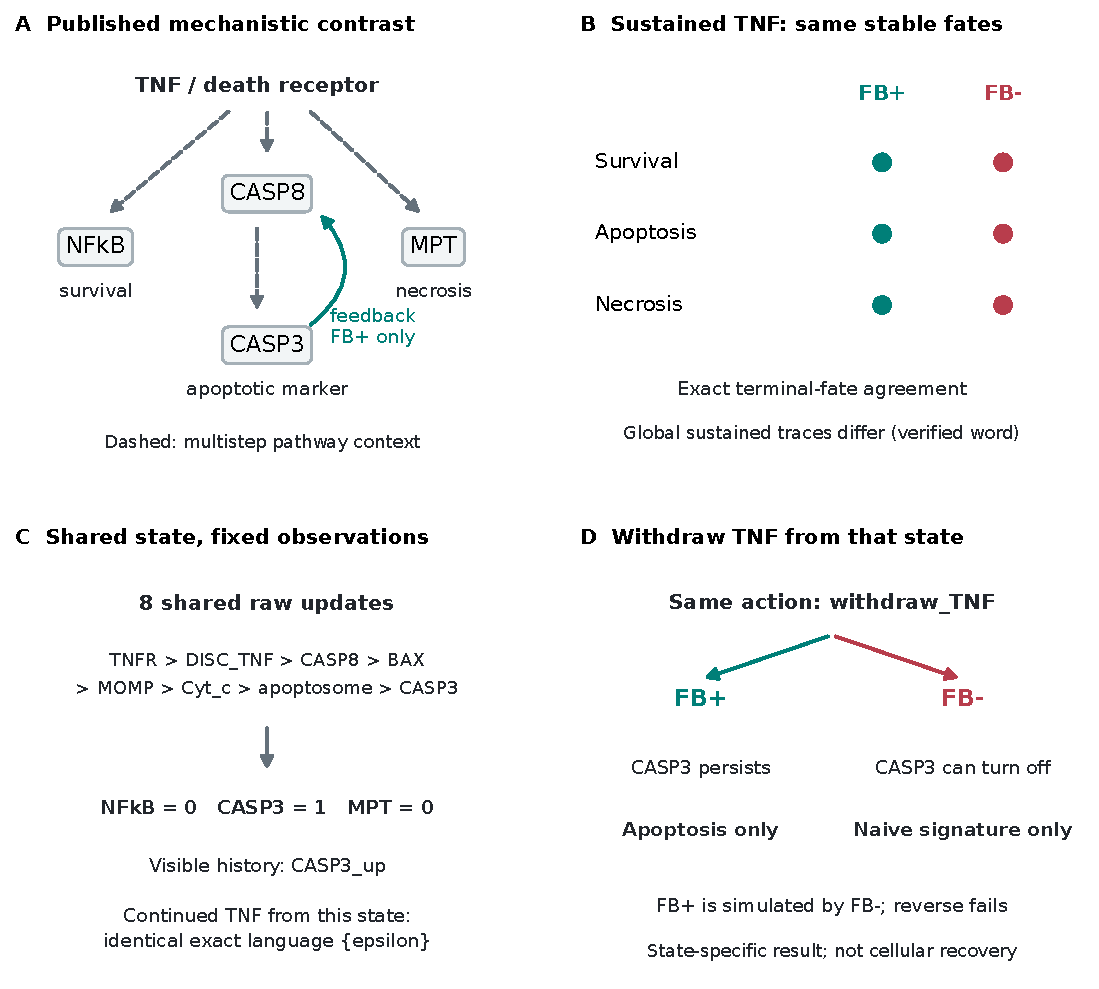
\includegraphics[width=\textwidth]{R3_Fig1.pdf}
\caption{Fixed-interface commitment comparison. (A) Mechanistic context, with
the literature-described CASP3-to-CASP8 feedback highlighted; dashed connectors
summarize multistep pathways, not direct molecular interactions.
(B) Both sustained-stimulation models reach the same three stable fates.
(C) An automatically extracted common history reaches the same retained
state; with continued TNF, both continuations have language $\{\epsilon\}$.
(D) Withdrawal from that state yields persistent CASP3 and an apoptotic
terminal fate for DR-FB+, but permits CASP3 loss and only the naive terminal
signature for DR-FB-. Counts and relations refer to exact retained-state
executions. No event count is converted to physical time.}
\label{fig:death-commitment}
\alttext{Four panels show the feedback hypothesis, matching baseline fates,
a shared CASP3-positive history, and different TNF-withdrawal continuations.}
\end{figure}

\subsection{A common history and a state-specific commitment witness}

The deterministic breadth-first search selects the first shared reachable state
satisfying persistent CASP3 and a unique apoptotic terminal future after
withdrawal in DR-FB+, versus a unique naive terminal future in DR-FB-.
One shortest raw-update path to this state is
\[
\begin{split}
&\mathrm{TNFR}\!\uparrow,\ \mathrm{DISC\_TNF}\!\uparrow,\
\mathrm{CASP8}\!\uparrow,\ \mathrm{BAX}\!\uparrow,\
\mathrm{MOMP}\!\uparrow,\\
&\mathrm{Cyt\_c}\!\uparrow,\ \mathrm{apoptosome}\!\uparrow,\
\mathrm{CASP3}\!\uparrow .
\end{split}
\]
All eight updates and the resulting retained vector are available in both
variants. The visible projection is $h=\texttt{CASP3\_up}$.
At this state, TNF, FADD, ATP, cIAP, TNFR, DISC\_TNF, CASP8, BAX, MOMP,
Cyt\_c, apoptosome and CASP3 are one; all other retained components are zero.
Thus the selected state is fully specified, not merely a pair of matching
marker values. The automatic selection is minimal in raw-event depth among
the states satisfying this criterion; it is not a claim of a globally shortest
biological observation or of a unique commitment state.

When withdrawal is permitted from this state, the continuations have
\DRLocalPlusStates{} states/\DRLocalPlusEdges{} edges and
\DRLocalMinusStates{} states/\DRLocalMinusEdges{} edges, respectively.
Write them $K_+$ and $K_-$. Exact checks give
\[
 K_+\weakpre K_-,\qquad K_-\not\weakpre K_+,\qquad
 K_+\not\weaksim K_-.
\]
The distinguishing trace in $K_-$ is
$\texttt{withdraw\_TNF}\,\texttt{CASP3\_down}$, absent from $K_+$.
The independent deletion-game certificate covers every defending weak reply,
not one conveniently chosen successor. Its dependency ranks decrease until
CASP3 deactivation has no matching action. Production predicates and mCRL2
agree on bisimulation and exact traces; both simulation directions are also
checked by the independent game.

The direction is important: $K_-$ can match the fewer observable actions of
$K_+$, but $K_+$ cannot match the additional deactivation response of $K_-$.
This is not a ranking of biological quality or survival. After immediate
withdrawal, $K_+$ retains CASP3 along every continuation and reaches only
apoptosis, whereas $K_-$ reaches only the model's naive signature. The latter
is a marker-level logical outcome, not evidence that an apoptotic cell can
return to viability.

\subsection{What the shared observation does and does not identify}

The visible history $h$ alone is compatible with \DRHistoryStates{} hidden
states in each sustained model. Aggregating complete post-withdrawal futures
over all such states gives
\[
\begin{split}
\mathrm{Futures}_+(h,\mathrm{withdraw})
 &=\{\mathrm{apoptosis},\mathrm{naive},\mathrm{necrosis}\},\\
\mathrm{Futures}_-(h,\mathrm{withdraw})
 &=\{\mathrm{naive},\mathrm{necrosis}\}.
\end{split}
\]
Therefore the difference is not confined to an arbitrarily paired pair of
hidden states. However, $h$ does not imply that every compatible DR-FB+ state
is irreversibly apoptotic. The full state witness and the history-aggregated
future sets answer different questions and are reported separately.

The complete withdrawal-aware systems have \DRControlPlusStates{} and
\DRControlMinusStates{} reachable states. Exact subset propagation gives a
DR-FB--only trace
$\texttt{CASP3\_up}\,\texttt{withdraw\_TNF}\,\texttt{CASP3\_down}$;
the defending DR-FB+ subset is empty after its last action. A trace in the
opposite direction is
$\texttt{withdraw\_TNF}\,\texttt{CASP3\_up}\,\texttt{CASP3\_down}\,
\texttt{CASP3\_up}$.
These exact counterexamples refute both global trace inclusions and hence both
global weak-simulation directions; they require no exhaustive language
enumeration. Ordinary trace comparison can detect differences under both the
sustained and withdrawal protocols. We do not present this biological
case as the stronger equal-global-trace/different-branching phenomenon of
Example~\ref{ex:branching}.

The exhaustive scan considers every reachable history of exactly $k$ raw
updates before withdrawal, for $0\leq k\leq40$, with complete future
reachability thereafter. An apoptotic terminal future first becomes possible
in DR-FB+ after one hidden TNFR update; persistent-CASP3 commitment first appears
at $k=\DRDepth{}$, for \DRFirstCommitted{} of \DRDepthStates{} reachable
states at that depth. It never occurs in DR-FB- over this scan. State counts
are not path probabilities. No artificial stutters are added at terminal
states, no physical duration is assigned, and this first possible depth is
not a universal time at which all modeled cells commit.

\subsection{Prospective discriminator and evidential status}

The model-derived discriminator is a pulse/withdrawal comparison at a
CASP3-positive stage, followed by the joint observation of CASP3 persistence,
NFkB activity and MPT, with ATP status supporting fate classification.
Monitoring the other two markers matters: CASP3 loss accompanied by a change
in the necrotic branch is not the same trace as isolated CASP3 loss after
withdrawal. The three-marker history does not uniquely locate the hidden
witness state; more detailed state assessment would be needed to test its
state-specific claim. We specify no concentration, cell line, elapsed time or
selective experimental feedback inhibitor that these logical models cannot
justify. Ligand withdrawal and the feedback hypothesis originate in the
Calzone study.\cite{Calzone2010} Our added result is the explicit relational
and reachable-future account, not a newly proposed biological mechanism.

\begin{table}[t]
\tbl{Specified assumptions, computed results, and absent evidence in the
death-receptor comparison.\label{tab:evidence-status}}{
\small\setlength{\tabcolsep}{4pt}
\begin{tabular}{@{}>{\raggedright\arraybackslash}p{0.31\textwidth}>{\raggedright\arraybackslash}p{0.64\textwidth}@{}}
\toprule
Item & Evidential status\\
\colrule
CASP3-to-CASP8 feedback & Published model assumption; its removal was already studied.\\
Markers and withdrawal & Fixed interface and intervention declared before relation results.\\
Baseline terminal fates & Computed agreement: survival, apoptosis, necrosis.\\
Shared-state continuations & Exact sustained equality; one-way simulation and unequal traces with withdrawal.\\
Global sustained traces & Equality refuted by a verified 12-action word; reverse inclusion undecided.\\
Witness and fate persistence & Automatically computed; all defending replies checked.\\
Discriminating observation & Model-derived implication of a published perturbation.\\
Wet-lab confirmation & No new experimental validation; naive is not demonstrated cellular recovery.\\
\botrule
\end{tabular}}
\end{table}

\section{GIM illustration: interface-conditioned behavioral correspondence}\label{sec:gim-results}

\subsection{Structure held constant}
The animal and plant nets reach 13 and 14 states, respectively. No place,
transition, arc, or initial marking changes across the three interfaces.
Native PN-GDDA is 0.9975846 throughout (0.9975175 with the independently
derived 576-orbit partition). This describes nearly identical selected local
wiring, not mechanistic identity or execution equivalence. Figure
\ref{fig:gim-interface} makes the comparison's biological assumptions and
computed outcomes visible together.

\begin{figure}[t]
\centering
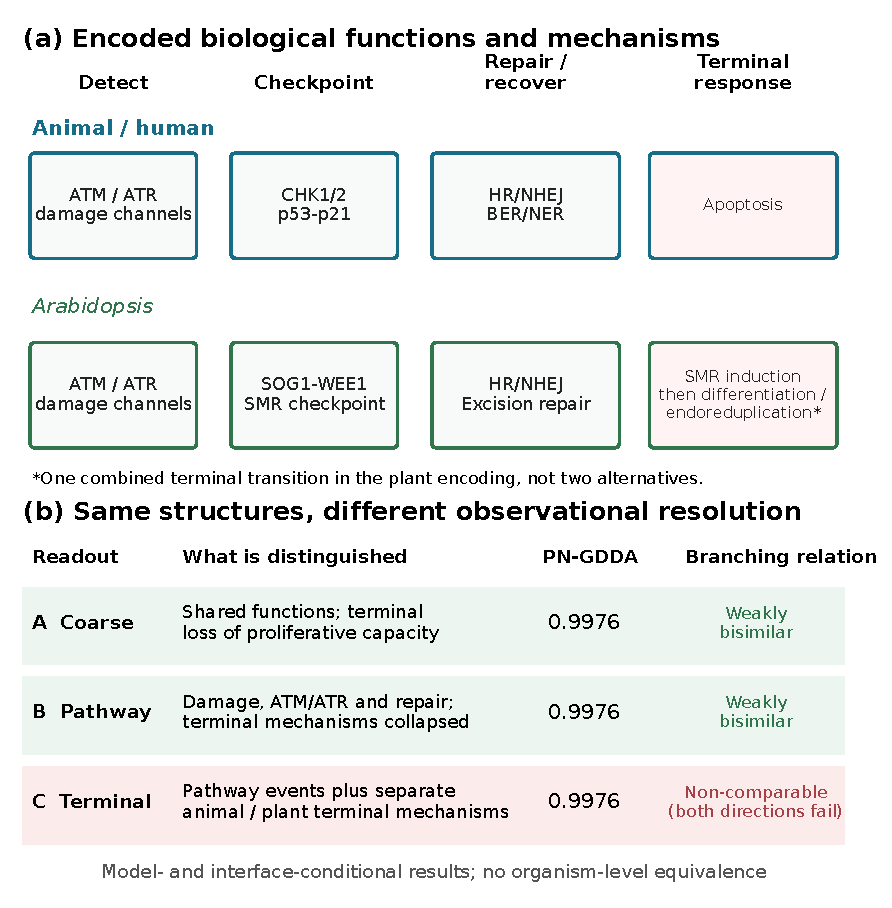
\includegraphics[width=\textwidth]{R3_Fig2.pdf}
\caption{Central GIM comparison. Upper-panel columns align encoded
animal/human and \tas{} functional categories; they are not a causal pathway
or a required sequence of outcomes. The lower panel
shows what each declared interface observes and the computed branching
relation. PN-GDDA remains 0.9976 because the structures are unchanged.
The combined plant terminal transition does not distinguish differentiation
from endoreduplication. Shared labels at A/B express a functional abstraction,
not identity between p53 and SOG1 or between terminal mechanisms.}
\label{fig:gim-interface}
\alttext{Animal and Arabidopsis damage-response functions above a three-row
interface comparison: A and B are weakly bisimilar; C is non-comparable,
with structural similarity constant at 0.9976.}
\end{figure}

\subsection{Coarse function retains correspondence}
At Interface A, every observable detection, checkpoint, repair, restoration,
or cycle-exit step in either executable model can be matched by the other,
with this matching preserved at the resulting states. Internal relays can
require different numbers of steps. Formally, the systems are weakly but not
strongly bisimilar. The result licenses comparison at the declared shared
functional level; it does not identify their molecular implementations.

\subsection{Pathway distinctions do not yet break the relation}
Interface B distinguishes damage channels, ATM/ATR-associated signaling, and
broad repair families. The models still match recursively when terminal
loss of proliferative capacity remains a common observation. Both simulation
directions and weak bisimilarity hold; strong bisimilarity does not.
Thus, among these encodings and interfaces, distinguishing those pathway
events alone is insufficient to eliminate the correspondence.

\subsection{Terminal mechanisms eliminate both directions}
At Interface C, mammalian \texttt{apoptosis} and plant
\texttt{smr\_induction} followed by
\texttt{differentiation\_or\_endoreduplication} become distinct observations.
Neither model can match all observable moves of the other, so weak
bisimilarity and both simulation directions fail. This is not an unexpected
biological discovery: the terminal labels intentionally encode prior knowledge
of different mechanisms. The computational result confirms where, in the
tested sequence of readouts, that distinction prevents recursive matching.
The depth-six trace distance becomes 0.3529 rather than zero; LTS-GDA changes
from 0.9508 to 0.8921. These diagnostics accompany the formal decision, not
replace it (Table~\ref{tab:gim-sensitivity}).

\begin{table}[t]
\tbl{Recomputed GIM results. Animal$\preceq$Plant means that the plant model
simulates the animal model; Plant$\preceq$Animal is the reverse.
Strong bisimilarity is false throughout.\label{tab:gim-sensitivity}}{
\begin{tabular}{@{}lccp{1.10in}rr@{}}
\toprule
Interface & Animal$\preceq$Plant & Plant$\preceq$Animal & Class & $d_6$ & PN-GDDA\\
\colrule
A: coarse & Y & Y & weak bisimulation & 0.0000 & 0.9976\\
B: pathway & Y & Y & weak bisimulation & 0.0000 & 0.9976\\
C: terminal & N & N & non-comparable & 0.3529 & 0.9976\\
\botrule
\end{tabular}}
\end{table}

\subsection{What changes when observability changes?}
Interfaces A and B aggregate terminal mechanisms into a shared functional
readout, whereas C separates them. The first loss of correspondence is therefore
\emph{between B and C within this declared interface family}, not a uniquely
identified or globally minimal biological resolution. There is no exhaustive
search over all possible interfaces, and no experimental threshold is inferred.
The constant structural score isolates observability from topological change.

Prior biology supplies the distinct terminal mechanisms; PN-GDDA describes
their selected wiring; the executable comparison determines whether a
recursive correspondence survives each declared readout. Whether such a
model-level boundary predicts a cross-species experimental boundary remains
unvalidated. One testable interpretation is that readouts aggregating terminal
loss of proliferative capacity may preserve an apparent correspondence that
mechanism-specific readouts do not. This is a model-derived hypothesis, not an
assay result. The full Petri nets remain in \ref{app:gim-nets}.

\section{Supporting and exploratory comparisons}\label{sec:case-method}

Five compact plant--animal pairs encode DNA repair/genome instability (GIM), energy
metabolism (DCE), cell-cycle control (SPS), cell death/autophagy (RCD), and
immune control (AID). Comparative studies and cancer-hallmark literature guided
component selection; dedicated reviews informed plant DNA-damage, cell-cycle,
and autophagy mechanisms.\cite{Quimbaya2012,ClavijoBuritica2023,Hanahan2022,
Yoshiyama2013} Transition-level provenance is machine-checked, which establishes
where encoded assumptions came from and whether documentation is complete. It
does not establish that the nets reproduce independent experiments. These
manually curated models contain no kinetics, concentrations, tissue context, or
independent experimental calibration.

The ten nets produced 5--14 reachable states. The GIM row in
Table~\ref{tab:case} reports Interface A; GIM, DCE, and SPS were weakly but
not strongly bisimilar; RCD gave plant-in-animal one-way simulation; AID was
non-comparable. Table~\ref{tab:case} juxtaposes these classes with native
PN-GDDA. The 592- and 576-orbit variants changed no score by 0.001 and no
threshold decision: all five pairs were structurally similar at 0.9 despite
three different behavioral classes.

\begin{table}[t]
\tbl{Supporting curated model-pair outputs. GIM is reported at Interface A;
all relations and $d_6$ values are interface-conditional, whereas PN-GDDA is
structural.\label{tab:case}}{
\begin{tabular}{@{}l>{\raggedright\arraybackslash}p{1.05in}>{\raggedright\arraybackslash}p{1.05in}rrr@{}}
\toprule
Module & Process & Formal class & $d_6$ & PN-592 & Orbit-576 \\
\colrule
GIM & DNA repair & weak bisimulation & 0.000 & 0.9976 & 0.9975 \\
DCE & energy metabolism & weak bisimulation & 0.000 & 0.9969 & 0.9968 \\
SPS & cell-cycle control & weak bisimulation & 0.000 & 1.0000 & 1.0000 \\
RCD & death/autophagy & plant in animal & 0.143 & 1.0000 & 1.0000 \\
AID & immune control & non-comparable & 0.429 & 0.9907 & 0.9904 \\
\botrule
\end{tabular}}
\end{table}

RCD supplies a secondary directional result: both encoded nets contain stress,
mTOR inhibition, autophagy, and survival, but only the animal encoding exposes a
canonical caspase-apoptosis branch; the plant branch uses an internal metacaspase
event. The plant LTS is weakly simulated by the animal LTS, whereas the reverse
direction fails. This means containment only for the declared labels of these
two models; it does not equate plant programmed cell death with mammalian
apoptosis. Silent subdivision preserved every class over 300 refinements per
module, while targeted relabeling changed the expected relations. Distances
against 2,000 label permutations assess internal interface sensitivity, not
external biological significance. DCE, SPS, and AID are retained as supporting
model-ingestion and relation-diversity examples rather than independent
biological validation.

\subsection{Exploratory confrontation with HPN-DREAM data}\label{sec:hpn-method}

An independent-data check is retained as a secondary, exploratory analysis,
not as validation of the GIM resolution boundary. Public HPN-DREAM/CASPOTS
families contain 72 BT20, 191 BT549, and 21 MCF7 Boolean networks.
Structure-only medoid selection, fixed before test-response access, chooses
zero-based rows 24, 137, and 9.\cite{Hill2016,Razzaq2018} The common interface
contains seven measured PI3K/MAPK/mTOR readouts under three shared held-out
mTOR-inhibitor conditions. Initial values, clamping, and update conventions
are specified in Supplementary Validation, Section~S3.

The nine asynchronous pair--condition comparisons contain six one-way
simulations and three non-comparable pairs. The six directions comprise three
left-model-in-right-model and three right-model-in-left-model relations, not
positions on an ordinal similarity scale. Direction is preserved in the result
fields; no scalar formal-class test is performed. Median profile RMSE is
0.2757, 0.1919, and 0.2071 in those three nominal categories, respectively,
with only three observations per category. Synchronous updating preserves
seven of the nine classes. These summaries cannot establish predictive value.

The retained continuous diagnostics are inconclusive: truncated-trace distance
has Spearman $\rho=-0.596$, exact one-sided $p=0.556$; LTS-GDA distance has
$\rho=0.669$, $p=0.097$, using all 216 condition-stratified permutations.
The CASPOTS native-context advantage over cross-cell medoids is 0.00212
excess-RMSE units and is not established by the exact three-cell sign test
($p=0.25$). No more favorable statistic was substituted. The full methods,
negative results, and plot remain in Supplementary Validation, Section~S3;
they show a route to data confrontation without claiming prognosis, native
cell-line specificity, or experimental equivalence.

\section{Supporting formal and implementation checks}
\label{sec:computational-validation}

Definitions and the executed relation-deletion method are supported by the
proofs in \ref{app:formal}. Table~\ref{tab:validation-summary} states
the checks, independent bases, and observed outcomes in the main article.
These checks address whether the implemented relations and structural score
behave as specified; they do not establish biological validity.

\begin{table}[!htbp]
\tbl{Main implementation-verification results. Agreement refers to the declared
inputs and predicates, not predictive accuracy on biological data.
\label{tab:validation-summary}}{
\small
\setlength{\tabcolsep}{4pt}
\renewcommand{\arraystretch}{1.08}
\begin{tabular}{@{}>{\raggedright\arraybackslash}p{0.205\textwidth}%
>{\raggedright\arraybackslash}p{0.37\textwidth}%
>{\raggedright\arraybackslash}p{0.37\textwidth}@{}}
\toprule
Check & Independent basis and scope & Observed result \\
\colrule
Constructed cases & Six pairs with classes fixed before classification & 6/6 classes and 6/6 binary weak-equivalence decisions recovered. \\
External equivalence & mCRL2 on six synthetic, six public-model controls, and nine HPN pairs & 42/42 strong/weak-bisimilarity decisions agree. \\
Directional audit & Raw-edge attacker--defender game on 32 model pairs and three hierarchy witnesses & No disagreement on either weak-simulation direction or strong/weak bisimilarity. \\
Exhaustive finite check & All 260 one-/two-state LTSs over $\{a,\tau\}$; 67,600 ordered pairs & No simulation or weak-bisimulation discrepancy; no hierarchy or trace-inclusion violation. \\
Structural score & Holmes 1.1.1: 151 graphlets, 592 slots; four-node net and one-arc-deletion control & PN-GDDA agrees to 12 decimal places; absolute difference $3.33\times10^{-16}$. \\
\botrule
\end{tabular}}
\end{table}

The public cell-cycle and p53--Mdm2 controls test SBML-qual and GINML imports;
all six copy, silent-refinement, and label-perturbation controls recover their
predeclared outcomes.\cite{Naldi2018,Chaouiya2013SBML,Traynard2016,AbouJaoude2009}
Holmes supplies an external reference for the PN-GDDA implementation.
\cite{Radom2017} mCRL2 supplies the external equivalence checks.
\cite{Bunte2019} Its simulation-preorder checks are used only for the two
tau-free hierarchy witnesses, where strong and weak simulation coincide;
no general weak-preorder verification is attributed to that tool.

For directional checks, the independent game constructs weak targets directly
from raw edges without calling the production closure or relation routines.
The 32 pairs comprise six synthetic, three GIM-interface, five curated, and
18 asynchronous/synchronous HPN comparisons. The exhaustive universe fixes
initial state zero and enumerates every edge subset; it is not a proof for
arbitrary finite systems. In particular, Example~\ref{ex:branching} separately
establishes early-to-late simulation, failure of the reverse, and exact trace
equality using an explicit witness and a failed-successor argument. No exact
trace conclusion is inferred from a truncated distance.

The evidence layers remain distinct: proofs establish mathematical claims;
tests establish implementation agreement on tested inputs; model provenance
and import checks establish executable assumptions; biological literature and
held-out data support or limit biological interpretation. Formal agreement alone
does not calibrate a curated net against experiments. Supplementary Validation
S1--S2 and S4 retain per-case outputs, comparator definitions, tool procedures,
and scaling details; the main death-receptor evidence is in Section~4 and GIM in Section~5.


The new death-receptor checks distinguish global from conditioned comparisons.
Compact Boolean execution is checked against the tuple-based executor;
the selected full 28-node continuations reproduce the quotient's weak results.
The exact conditioned sustained languages agree, while withdrawal gives one-way
simulation, confirmed by a raw-edge game certificate covering every defender
reply. mCRL2 independently confirms all six strong/weak/trace equivalence
decisions across the two conditioned protocols. Global withdrawal simulations
are refuted by exact trace counterexamples in both directions. An
independent tuple/product search using all 28 original rule callbacks
confirms acceptance in one variant and exhaustive rejection in the other for
each withdrawal counterexample, without compact storage or sink reduction.
Global sustained trace equality is also refuted: a 12-action word is possible
only in DR-FB+, as independently checked by sparse reachability and mCRL2.
A reconstructed 53-update accepting path satisfies the original full-model
rules. The reverse sustained inclusion remains undecided. The expanded
subset search still reaches its storage cap, but the finite witness suffices
to disprove equality; this is not an inference from resource exhaustion.
Supplementary Validation S5 gives the reduction argument, full graph sizes,
execution limits and event-depth scan. These limits are not counted as
failed equivalences or as successful biological validations.

\section{Discussion}\label{sec:discussion}

\subsection{Can commitment matter when ordinary predictions agree?}

The death-receptor case gives a qualified but concrete answer. The two
variants share their sustained stable-fate set. At an automatically located
shared state, even their complete sustained observable continuations agree,
yet ligand withdrawal exposes different persistent marker behavior and terminal
futures. This separates endpoint agreement from intervention-conditioned
commitment using a fixed biological interface. The analysis connects a
literature-derived mechanism to an explicit history, retained state, and
recursive-matching certificate instead of relying on relabeled terminal
mechanisms.

The scope must remain precise. Global sustained weak-trace equivalence is
refuted by a verified finite word, and the withdrawal-aware languages are
also unequal. The reverse sustained trace inclusion remains undecided.
The biological example consequently does not show that bisimulation discovers
a difference invisible to every trace-based comparison. Its value is the
systematic characterization of where matching fails and which futures remain
available under an intervention. The exact equal-trace/unequal-branching
phenomenon remains established by the accepted synthetic example; a biological
instantiation of that stronger property is still an open extension.

Nor do the markers uniquely identify a hidden commitment state. Although the
same visible prefix has different aggregated future sets in the two models,
it is compatible with \DRHistoryStates{} internal states in each. Presenting
one state-specific certificate as an unconditional prediction for every
CASP3-positive cell would erase the very nondeterminism the comparison is
intended to respect. The model's naive terminal signature after CASP3 loss
must also not be read as actual reversal of executed apoptosis. Downstream
irreversible damage, cell-type specificity and quantitative kinetics are not
established by this qualitative reconstruction.

Calzone et al. already analyzed feedback-dependent persistence under transient
ligand exposure.\cite{Calzone2010} Recovering that result is a use-case validation
of the relational workflow, not independent discovery or experimental
confirmation. The asymmetric simulation result adds an explicit account of
which continuation fails to match; the fate analysis supplies its biological
interpretation. These are complementary outputs, not interchangeable measures.

\subsection{Can changing the interface change correspondence?}

GIM addresses this separate methodological question. PN-GDDA characterizes
label-blind local Petri-net topology,\cite{Szawulak2022} whereas the executable
relations depend on labels, initial markings, and reachable choices. For the
unchanged GIM nets, weak correspondence persists at Interfaces A and B and
is lost at C, the first tested interface exposing the known terminal
distinction. This result is limited to those three declared readouts; there is
no exhaustive interface search, unique biological boundary, or globally minimal
resolution claim. The distinct terminal biology was encoded in advance, not
discovered by formal comparison.

The two cases must not be conflated. GIM changes observability while holding
the models fixed. The death-receptor study holds the interface fixed and
compares a documented mechanistic variant under sustained and withdrawal
protocols. PN-GDDA is retained for the former structural question; no uncomputed
PN-GDDA score is assigned to the death-receptor models.

\subsection{Validation, execution assumptions and limits}

The accepted mathematical development, direction conventions, and fixed-point
algorithm are unchanged. Formal regression tests establish computational
correctness under declared semantics, not biological adequacy. The new analysis
adds independent compact/tuple execution checks, a checked hidden-sink
reduction, full-model verification of the selected continuation, exact subset
counterexamples, and mCRL2 checks of the local equivalences and the sustained
counterexample word. State-space and
memory limits remain visible results, not negative relation decisions.

Unitary asynchronous updates encode possible orders, not calibrated rates.
Reachable terminal fates and marker persistence are distinguished from
inevitability under unrestricted scheduling. The selected post-withdrawal
continuations are acyclic, but no general fairness conclusion is inferred for
the much larger global graphs. Resource amendments change storage and remove
only proven irrelevant hidden readouts; they do not retune the biological
interface after inspecting relation outcomes. The prospective configuration
record is local, not an externally registered protocol or proof of absence
of analytic bias.

The HPN-DREAM/CASPOTS confrontation remains exploratory and its weak evidence
does not become stronger because the death-receptor example was added.
Likewise, the compact curated networks are not full organism-level pathways.
Future work should test other independently authored commitment models,
resolve the global sustained relations where feasible, and use state-resolved
experimental observations to challenge the predicted intervention responses.

\section{Conclusion}\label{sec:conclusion}

Endpoint-matched qualitative cell-fate models can differ in their responses to
signal withdrawal. With a fixed interface, the death-receptor feedback variants
share a reachable CASP3-positive state with exactly equivalent sustained
continuations but unequal withdrawal continuations and different terminal
futures. An automatic certificate explains the failed matching action and
preserves the simulation direction. This is a model-level reconstruction of a
published commitment phenomenon, not a new mechanism, proof of global
trace-equivalent biological branching, or wet-lab validation. GIM remains a
complementary illustration of the first correspondence loss among three
declared interfaces. Together, the cases separate what is specified through
models and readouts from what relational and reachable-future calculations
actually establish.

\appendix
\section{Mathematical properties and quantifier audit}\label{app:formal}
\label{sec:fixed-point}

For $a\in\Sigma_{\TAU}$, let $D_a^i(x)=\{x':x\xrightarrow{a}_i x'\}$ and
$U=S_1\times S_2$. Define operators on $\powerset(U)$ by
\begin{align}
\Phi_{\preceq}(R)=\{(x,y)\in U:
 &\ \forall a,x'\in D_a^1(x)\ \exists y'\in W_a^2(y),
 (x',y')\in R\},\label{eq:sim-operator}\\
\Phi_w(R)=\{(x,y)\in\Phi_{\preceq}(R):
 &\ \forall a,y'\in D_a^2(y)\ \exists x'\in W_a^1(x),
 (x',y')\in R\},\label{eq:weak-bisim-operator}\\
\Phi_s(R)=\{(x,y)\in U:
 &\ \forall a,x'\in D_a^1(x)\ \exists y'\in D_a^2(y),
 (x',y')\in R,\nonumber\\
 &\ \forall a,y'\in D_a^2(y)\ \exists x'\in D_a^1(x),
 (x',y')\in R\}.\label{eq:strong-bisim-operator}
\end{align}

\begin{theorem}[Correctness of relation deletion]\label{thm:fixed-point}
For each $\Phi\in\{\Phi_{\preceq},\Phi_w,\Phi_s\}$, the operator is monotone.
The implemented algorithm starts with $R=U$, repeatedly deletes any currently
examined pair $z\notin\Phi(R)$, and stops after a complete pass with no deletion.
On finite LTSs it terminates and returns the greatest fixed point $\nu\Phi$.
Consequently, testing membership of $(s_1^0,s_2^0)$ computes, respectively,
weak simulation in the orientation of Definition \ref{def:weak-simulation}, weak
bisimilarity, and strong bisimilarity.
\end{theorem}

\begin{proof}
If $R\subseteq Q$, every witness pair in $R$ remains available in $Q$; hence
$\Phi(R)\subseteq\Phi(Q)$ for each operator. Every deletion strictly decreases
the finite relation, so termination requires at most $|U|$ deletions.

Let $G=\nu\Phi$. The invariant $G\subseteq R$ holds initially. If it holds before
a deletion and $z\in G$, then
$z\in\Phi(G)\subseteq\Phi(R)$, so $z$ cannot be deleted. Thus $G$ remains a
subset of the terminal relation $R_*$. A final pass without deletion gives
$R_*\subseteq\Phi(R_*)$. Conversely, each $z\notin R_*$ was deleted from some
$R_z$ with $z\notin\Phi(R_z)$. Since $R_*\subseteq R_z$, monotonicity implies
$\Phi(R_*)\subseteq\Phi(R_z)$ and therefore $z\notin\Phi(R_*)$. Hence
$R_*=\Phi(R_*)$. Because $R_*$ is a fixed point, $R_*\subseteq G$; together
with the invariant this yields $R_*=G$. The three operators are exactly the
transfer clauses of Definitions \ref{def:weak-simulation} and
\ref{def:bisimulation}.
\end{proof}

\begin{remark}[Resource bound]\label{rem:complexity}
Writing $n_i=|S_i|$, the candidate relation stores $O(n_1n_2)$ pairs and permits
at most $n_1n_2$ deletions and $n_1n_2+1$ passes. Each pass scans current pairs,
outgoing moves, and matching direct or weak targets. Silent closures are cached;
visible weak targets are constructed on demand. We therefore report these
parameters instead of claiming an unjustified tight time bound.
\end{remark}

\begin{proposition}[Hierarchy of behavioral relations]\label{prop:hierarchy}
For finite LTSs under Definitions \ref{def:weak-move}--\ref{def:weak-traces},
\begin{equation}\label{eq:hierarchy}
L_1\strongsim L_2
\Longrightarrow L_1\weaksim L_2
\Longrightarrow
(L_1\weakpre L_2\ \land\ L_2\weakpre L_1)
\Longrightarrow L_w(L_1)=L_w(L_2).
\end{equation}
The converses do not hold in general.
\end{proposition}

\begin{proof}
A direct match is a permitted weak match, and each direction of a weak
bisimulation is a weak simulation. If $L_1\weakpre L_2$, induction along any
finite concrete path matches observable moves by $\TAU^*a\TAU^*$ and silent
moves by $\TAU^*$, preserving related successors. Erasing $\TAU$ gives
$L_w(L_1)\subseteq L_w(L_2)$; the reverse simulation gives equality.
Proposition \ref{prop:silent-refinement} and Example \ref{ex:branching} refute
the first and last converses. For the middle converse, compare
$a.(b+c)+a.b$ with $a.(b+c)$: each simulates the other, but the $a.b$ successor
cannot be bisimilar to a state offering both $b$ and $c$.
\end{proof}


\begin{table}[t]
\tbl{Distinct witnesses for the three failed converses. All pairs have equal
exact weak-trace languages; $X\preceq Y$ means $Y$ simulates $X$.
\label{tab:hierarchy-witnesses}}{
\begin{tabular}{@{}p{1.75in}p{1.6in}p{1.3in}@{}}
\toprule
Converse refuted & Witness pair $(X,Y)$ & Decisive properties\\
\colrule
Weak implies strong bisimilarity & $a.0$, $a.\tau.0$ & weak, not strong\\
Mutual simulation implies weak bisimilarity & $a.(b+c)+a.b$, $a.(b+c)$ & both directions, not weak\\
Exact trace equality implies mutual simulation & late choice, early choice & early$\preceq$late only\\
\botrule
\end{tabular}}
\end{table}

For the middle row, write $x_{bc},x_b$ for the two $a$-successors of $X$ and
$y_{bc}$ for the sole $a$-successor of $Y$. A simulation from $X$ to $Y$
relates both $x_{bc}$ and $x_b$ to $y_{bc}$, with corresponding terminal
pairs. A simulation from $Y$ to $X$ relates $y_{bc}$ only to $x_{bc}$.
Both initial pairs therefore survive. A bisimulation would additionally need
to match $X$'s transition to $x_b$ with $y_{bc}$; the latter's $c$-move has
no counterpart at $x_b$. This witness concerns only the middle converse,
not the trace-equality converse refuted by Example~\ref{ex:branching}.

\begin{proposition}[Controlled silent edge refinement]
\label{prop:silent-refinement}
Let $L$ contain $p\xrightarrow{a}q$ with $a\in\Sigma$ and $p\neq q$. Construct
$L'$ by copying all original states and transitions except this edge, and replacing
it by
\begin{equation}\label{eq:silent-refinement}
 \bar p\xrightarrow{a}r\xrightarrow{\TAU}\bar q,
\end{equation}
where $r$ is fresh and has no other incident behavior. Then $L\weaksim L'$.
Repeated refinements of this form also preserve weak bisimilarity. If $p$ and
$\bar p$ are initial, the selected edge is the only $a$-edge from $\bar p$ in
$L'$, and every $a$-successor of $p$ in $L$ has no outgoing $\TAU$ transition,
then $L\not\strongsim L'$.
\end{proposition}

\begin{proof}
Let
$R=\{(x,\bar x):x\in S\}\cup\{(q,r)\}$. For every copied pair other than the
source, direct moves are copied. At $(p,\bar p)$, the original edge is matched
by $\bar p\xrightarrow{a}r\xrightarrow{\TAU}\bar q$, while
$\bar p\xrightarrow{a}r$ is matched by $p\xrightarrow{a}q$ and ends in
$(q,r)$. At $(q,r)$, moves from $q$ are matched after
$r\xrightarrow{\TAU}\bar q$; that silent move is itself matched by zero silent
moves at $q$. Hence $R$ is a weak bisimulation, and repetition follows by
transitivity. Under the additional conditions, a strong match for
$\bar p\xrightarrow{a}r$ must relate $r$ to an $a$-successor $x$ of $p$, but
$r\xrightarrow{\TAU}\bar q$ would require the excluded direct $\TAU$-move from
$x$. Thus strong bisimilarity fails.
\end{proof}

\begin{proposition}[Limit of label-blind structural comparison]
\label{prop:label-blind}
Let $M$ be any comparator determined only by unlabeled structure and invariant
under relabeling of transitions. Then $M$ cannot characterize weak-trace
equality, weak simulation or weak bisimilarity for labeled systems in general.
\end{proposition}

\begin{proof}
Take two systems with the same two states and one directed edge. Label the edge
$a$ in $L_a$ and $b\neq a$ in $L_b$. Their unlabeled structures are identical,
so $M(L_a,L_b)=M(L_a,L_a)$. Yet their languages are
$\{\epsilon,a\}$ and $\{\epsilon,b\}$, and neither observable move can be
matched by the other system. Thus no decision based only on $M$ can characterize
the stated labeled relations.
\end{proof}

Proposition \ref{prop:label-blind} does not identify a defect in PN-GDDA. It
states that a label-blind structural method answers a different question and
cannot substitute for a labeled behavioral relation.

\begin{example}[Equal traces, different branching]\label{ex:branching}
Let the late-choice system start at $\ell_0$ and have exactly
\begin{equation}\label{eq:late-choice}
\ell_0\xrightarrow{a}\ell_1,\qquad
\ell_1\xrightarrow{b}\ell_b,\qquad \ell_1\xrightarrow{c}\ell_c,
\end{equation}
and let the early-choice system start at $e_0$ and have exactly
\begin{equation}\label{eq:early-choice}
e_0\xrightarrow{a}e_b,\quad e_0\xrightarrow{a}e_c,\quad
e_b\xrightarrow{b}e'_b,\quad e_c\xrightarrow{c}e'_c.
\end{equation}
All unlisted states are terminal; neither system has silent transitions or
cycles. Enumerating all paths, whose lengths are at most two, gives both exact
prefix-closed languages as $\{\epsilon,a,ab,ac\}$, not merely a truncated match.

An explicit simulation from early to late is
\begin{equation}\label{eq:early-late-witness}
R_{E\to L}=\{(e_0,\ell_0),(e_b,\ell_1),(e_c,\ell_1),
(e'_b,\ell_b),(e'_c,\ell_c)\}.
\end{equation}
Both initial $a$-moves are matched by $\ell_0\xrightarrow{a}\ell_1$.
At $(e_b,\ell_1)$ the sole $b$-move has a match; at $(e_c,\ell_1)$ the sole
$c$-move has a match. Terminal pairs impose no further obligations. Thus
$L_{\mathrm{early}}\weakpre L_{\mathrm{late}}$.

Conversely, suppose a simulation $R$ from late to early contains
$(\ell_0,e_0)$. Matching the single transition
$\ell_0\xrightarrow{a}\ell_1$ requires choosing one successor of $e_0$ and
including the resulting pair in $R$. If $(\ell_1,e_b)\in R$, the $c$-move
from $\ell_1$ has no match. If $(\ell_1,e_c)\in R$, its $b$-move has no
match. These exhaust the possible $a$-successors, so no such $R$ exists:
$L_{\mathrm{late}}\not\weakpre L_{\mathrm{early}}$. Weak bisimilarity
therefore also fails.

Different outgoing transitions from a related pair may indeed choose different
matching successors. However, the \emph{one} initial late $a$-transition must
be matched by an early successor pair that itself satisfies every subsequent
transfer obligation. Trace matching may select the $e_b$ branch for $ab$ and
the $e_c$ branch for $ac$ independently; simulation cannot combine those two
states into one defender state after the initial move. This is the quantifier
distinction behind the final strictness claim of Proposition
\ref{prop:hierarchy}.
\end{example}

\section{Detailed GIM Petri-net encodings}\label{app:gim-nets}

Figures~\ref{fig:gim-animal-net} and \ref{fig:gim-plant-net} show the
fixed executable nets; the three interfaces change only transition labels.

\clearpage
\begin{sidewaysfigure}[p]
\centering
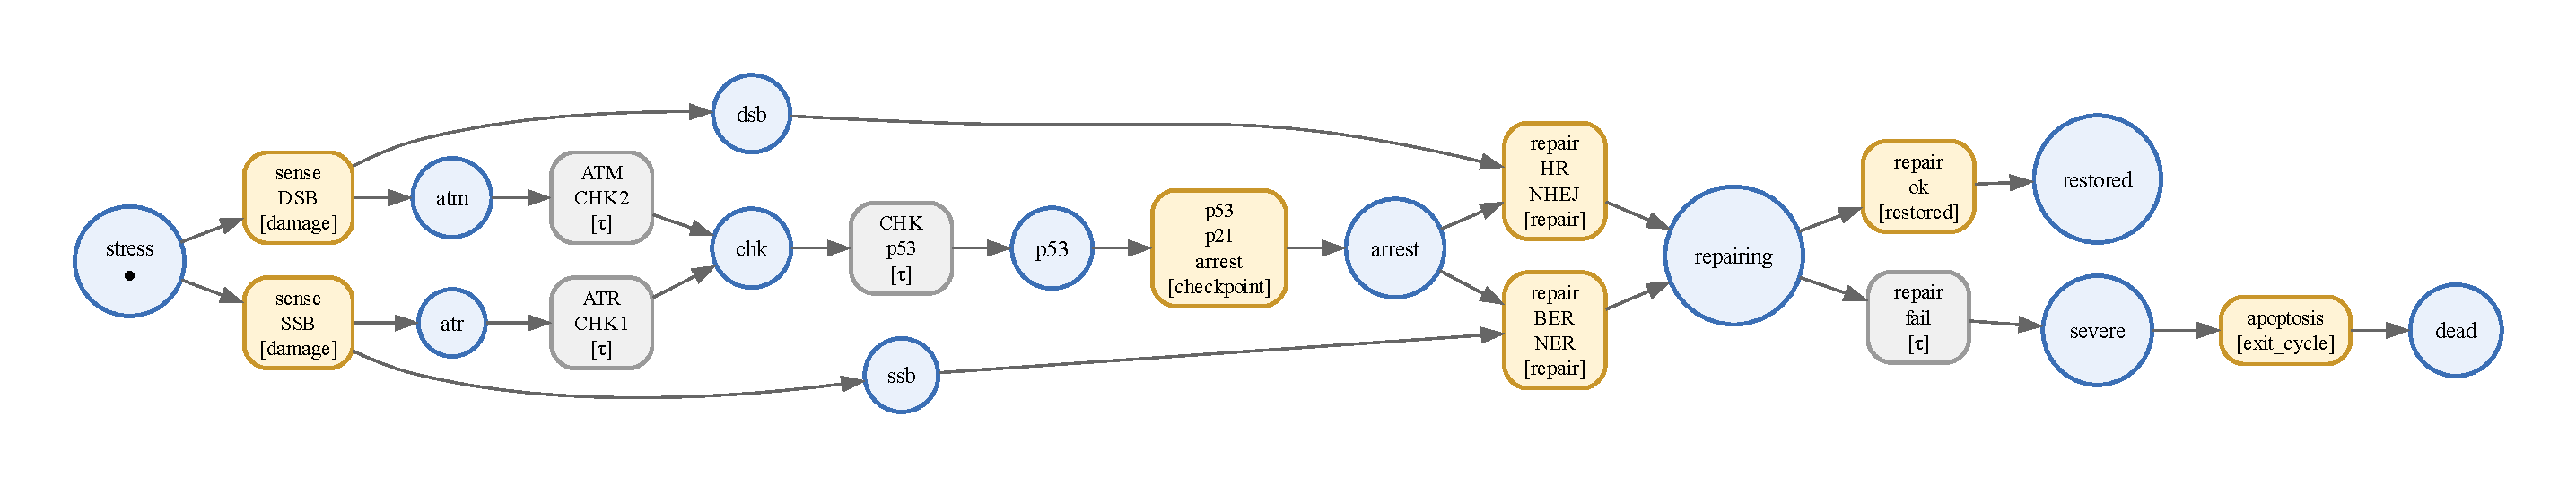
\includegraphics[width=0.94\textheight]{R3_Fig3.pdf}
\caption{Detailed animal/human GIM Petri net. Circles are places, rounded boxes
are transitions, brackets show the base/coarse observable labels, and gray
$\tau$ transitions are internal.}
\label{fig:gim-animal-net}
\alttext{Detailed animal and human DNA-damage Petri net with places,
transitions, labels, and arcs.}
\end{sidewaysfigure}

\begin{sidewaysfigure}[p]
\centering
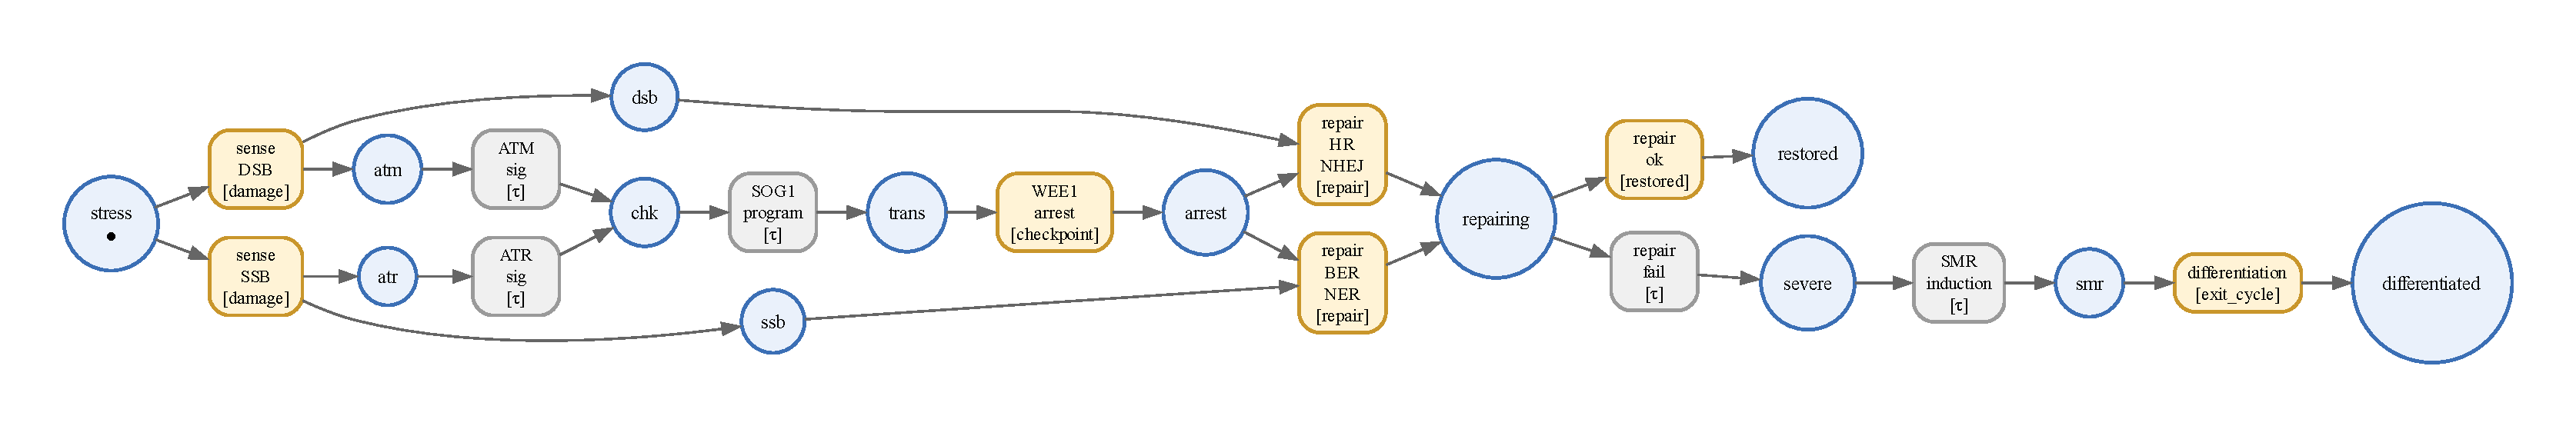
\includegraphics[width=0.94\textheight]{R3_Fig4.pdf}
\caption{Detailed \tas{} GIM Petri net, using the same graphical conventions as
Fig.~\ref{fig:gim-animal-net}. The terminal transition is a combined outcome in
this encoding and does not distinguish differentiation from endoreduplication.}
\label{fig:gim-plant-net}
\alttext{Detailed Arabidopsis DNA-damage Petri net with places, transitions,
labels, and arcs.}
\end{sidewaysfigure}

\clearpage

\section*{Data and code availability}

Code, curated definitions, hash-verified public models, normalized response
files, metadata, and generated results are available under the MIT License at
\url{https://github.com/cero1979/BisimulationMol}. The accompanying R3 reproducibility archive supplies the third-revision sources, executed notebook, exact continuation outputs, and execution protocol; these additions are not yet a separately published remote release.
The repository documents
formal/software verification, interface definitions, figure regeneration,
tests, and notebook execution. Machine-readable GIM and HPN results are provided
as \texttt{results/gim\_interface\_sensitivity.csv} and
\texttt{results/hpn\_dream\_formal\_data\_validation.csv}. No confidential or
participant-level data were used.

\section*{Declarations}

\noindent\textbf{Funding.} No specific funding was received.
\textbf{Competing interests.} The author declares no competing interests.
\textbf{Ethics.} Only computational models and published aggregate data were
used; no human participants, samples, or live animals were involved.
\textbf{Author contributions.} Carlos Ramirez Ovalle performed the
conceptualization, methodology, software, formal analysis, validation,
visualization, drafting, and revision.

\begin{thebibliography}{10}
\providecommand{\url}[1]{\texttt{#1}}
\providecommand{\urlprefix}{URL }
\expandafter\ifx\csname urlstyle\endcsname\relax
  \providecommand{\doi}[1]{doi:\discretionary{}{}{}#1}\else
  \providecommand{\doi}{doi:\discretionary{}{}{}\begingroup
  \urlstyle{rm}\Url}\fi

\bibitem{Calzone2010}
Calzone L, Tournier L, Fourquet S, Thieffry D, Zhivotovsky B, Barillot E,
Zinovyev A, Mathematical modelling of cell-fate decision in response to death
receptor engagement, \emph{PLoS Computational Biology} \textbf{6}(3):e1000702, 2010.
\newblock \doi{10.1371/journal.pcbi.1000702}.

\bibitem{ChaouiyaPetriBio2007}
Chaouiya C, Petri net modelling of biological networks, \emph{Briefings in
  Bioinformatics} \textbf{8}(4):210--219, 2007.
\newblock \doi{10.1093/bib/bbm029}.

\bibitem{Li2006}
Li C, Suzuki S, Ge QW, Nakata M, Matsuno H, Miyano S, Structural modeling and
  analysis of signaling pathways based on {Petri} nets, \emph{Journal of
  Bioinformatics and Computational Biology} \textbf{4}(5):1119--1140, 2006.
\newblock \doi{10.1142/S021972000600234X}.

\bibitem{Fisher2007}
Fisher J, Henzinger TA, Executable cell biology, \emph{Nature Biotechnology}
  \textbf{25}(11):1239--1249, 2007.
\newblock \doi{10.1038/nbt1356}.

\bibitem{Szawulak2022}
Szawulak B, Formanowicz P, Graphlets in comparison of {Petri} net-based models
  of biological systems, \emph{Scientific Reports} \textbf{12}:20942, 2022.
\newblock \doi{10.1038/s41598-022-24535-5}.

\bibitem{Milner1989}
Milner R, \emph{Communication and Concurrency}, Prentice Hall, New York, 1989.
\newblock ISBN 978-0-13-115007-2.

\bibitem{Sangiorgi2011}
Sangiorgi D, \emph{Introduction to Bisimulation and Coinduction}, Cambridge
  University Press, Cambridge, 2011.
\newblock ISBN 978-1-107-00363-7.
\newblock \doi{10.1017/CBO9780511777110}.

\bibitem{JacksonBartek2009}
Jackson SP, Bartek J, The {DNA}-damage response in human biology and disease,
  \emph{Nature} \textbf{461}(7267):1071--1078, 2009.
\newblock \doi{10.1038/nature08467}.

\bibitem{BlackfordJackson2017}
Blackford AN, Jackson SP, {ATM}, {ATR}, and {DNA-PK}: The trinity at the heart
  of the {DNA} damage response, \emph{Molecular Cell} \textbf{66}(6):801--817,
  2017.
\newblock \doi{10.1016/j.molcel.2017.05.015}.

\bibitem{Yoshiyama2013}
Yoshiyama KO, Sakaguchi K, Kimura S, Dna damage response in plants: conserved
  and variable response compared to animals, \emph{Biology}
  \textbf{2}(4):1338--1356, 2013.
\newblock \doi{10.3390/biology2041338}.

\bibitem{DeSchutter2007}
De~Schutter K, Joub{\`e}s J, Cools T, Verkest A, Corellou F, Babiychuk E, Van
  Der~Schueren E, Beeckman T, Kushnir S, Inz{\'e} D, De~Veylder L,
  {Arabidopsis} {WEE1} kinase controls cell cycle arrest in response to
  activation of the {DNA} integrity checkpoint, \emph{The Plant Cell}
  \textbf{19}(1):211--225, 2007.
\newblock \doi{10.1105/tpc.106.045047}.

\bibitem{Yi2014}
Yi D, Kamei CLA, Cools T, Vanderauwera S, Takahashi N, Okushima Y, Eekhout T,
  Yoshiyama KO, \emph{et~al.}, The {Arabidopsis} {SIAMESE-RELATED}
  cyclin-dependent kinase inhibitors {SMR5} and {SMR7} regulate the {DNA}
  damage checkpoint in response to reactive oxygen species, \emph{The Plant
  Cell} \textbf{26}(1):296--309, 2014.
\newblock \doi{10.1105/tpc.113.118943}.

\bibitem{Adachi2011}
Adachi S, Minamisawa K, Okushima Y, Inagaki S, Yoshiyama K, Kondou Y, Kaminuma
  E, Kawashima M, Toyoda T, Matsui M, Kurihara D, Matsunaga S, Umeda M,
  Programmed induction of endoreduplication by {DNA} double-strand breaks in
  {Arabidopsis}, \emph{Proceedings of the National Academy of Sciences}
  \textbf{108}(24):10004--10009, 2011.
\newblock \doi{10.1073/pnas.1103584108}.

\bibitem{Hill2016}
Hill SM, Heiser LM, Cokelaer T, Unger M, Nesser NK, Carlin DE, \emph{et~al.},
  Inferring causal molecular networks: Empirical assessment through a
  community-based effort, \emph{Nature Methods} \textbf{13}(4):310--318, 2016.
\newblock \doi{10.1038/nmeth.3773}.

\bibitem{Razzaq2018}
Razzaq M, Paulev{\'e} L, Siegel A, Saez-Rodriguez J, Bourdon J, Guziolowski C,
  Computational discovery of dynamic cell line specific boolean networks from
  multiplex time-course data, \emph{PLOS Computational Biology}
  \textbf{14}(10):e1006538, 2018.
\newblock \doi{10.1371/journal.pcbi.1006538}.

\bibitem{Ogita2018}
Ogita N, Okushima Y, Tokizawa M, Yamamoto YY, Tanaka M, Seki M, Makita Y,
  Matsui M, Okamoto-Yoshiyama K, \emph{et~al.}, Identifying the target genes of
  {SUPPRESSOR OF GAMMA RESPONSE 1}, a master transcription factor controlling
  {DNA} damage response in {Arabidopsis}, \emph{The Plant Journal}
  \textbf{94}(3):439--453, 2018.
\newblock \doi{10.1111/tpj.13866}.

\bibitem{ManovaGruszka2015}
Manova V, Gruszka D, {DNA} damage and repair in plants---from models to crops,
  \emph{Frontiers in Plant Science} \textbf{6}:885, 2015.
\newblock \doi{10.3389/fpls.2015.00885}.

\bibitem{FulcherSablowski2009}
Fulcher N, Sablowski R, Hypersensitivity to {DNA} damage in plant stem cell
  niches, \emph{Proceedings of the National Academy of Sciences}
  \textbf{106}(49):20984--20988, 2009.
\newblock \doi{10.1073/pnas.0909218106}.

\bibitem{Murata1989}
Murata T, Petri nets: Properties, analysis and applications, \emph{Proceedings
  of the IEEE} \textbf{77}(4):541--580, 1989.
\newblock \doi{10.1109/5.24143}.

\bibitem{Quimbaya2012}
Quimbaya M, Vandepoele K, Rasp{\'e} E, Matthijs M, Dhondt S, Beemster GTS, Berx
  G, De~Veylder L, Identification of putative cancer genes through data
  integration and comparative genomics between plants and humans,
  \emph{Cellular and Molecular Life Sciences} \textbf{69}(12):2041--2055, 2012.
\newblock \doi{10.1007/s00018-011-0909-x}.

\bibitem{ClavijoBuritica2023}
Clavijo-Buritic\'a DC, Sosa CC, C\'ardenas-Heredia R, Mosquera AJ, \'Alvarez A,
  Medina J, Quimbaya M, Use of {Arabidopsis thaliana} as a model to understand
  specific carcinogenic events: Comparison of the molecular machinery
  associated with cancer-hallmarks in plants and humans, \emph{Heliyon}
  \textbf{9}(4):e15367, 2023.
\newblock \doi{10.1016/j.heliyon.2023.e15367}.

\bibitem{Hanahan2022}
Hanahan D, Hallmarks of cancer: new dimensions, \emph{Cancer Discovery}
  \textbf{12}(1):31--46, 2022.
\newblock \doi{10.1158/2159-8290.CD-21-1059}.

\bibitem{Naldi2018}
Naldi A, Hernandez C, Abou-Jaoud\'e W, Monteiro PT, Chaouiya C, Thieffry D,
  Logical modeling and analysis of cellular regulatory networks with {GINsim}
  3.0, \emph{Frontiers in Physiology} \textbf{9}:646, 2018.
\newblock \doi{10.3389/fphys.2018.00646}.

\bibitem{Chaouiya2013SBML}
Chaouiya C, B\'erenguier D, Keating SM, Naldi A, van Iersel MP, Rodriguez N,
  \emph{et~al.}, {SBML} qualitative models: a model representation format and
  infrastructure to foster interactions between qualitative modelling
  formalisms and tools, \emph{BMC Systems Biology} \textbf{7}:135, 2013.
\newblock \doi{10.1186/1752-0509-7-135}.

\bibitem{Traynard2016}
Traynard P, Faur\'e A, Fages F, Thieffry D, Logical model specification aided
  by model-checking techniques: Application to the mammalian cell cycle
  regulation, \emph{Bioinformatics} \textbf{32}(17):i772--i780, 2016.
\newblock \doi{10.1093/bioinformatics/btw457}.

\bibitem{AbouJaoude2009}
Abou-Jaoud\'e W, Ouattara DA, Kaufman M, From structure to dynamics: Frequency
  tuning in the p53--mdm2 network, \emph{Journal of Theoretical Biology}
  \textbf{258}(4):561--577, 2009.
\newblock \doi{10.1016/j.jtbi.2009.02.005}.

\bibitem{Radom2017}
Radom M, Rybarczyk A, Szawulak B, Andrzejewski H, Chabelski P, Kozak A,
  Formanowicz P, Holmes: A graphical tool for development, simulation and
  analysis of {Petri} net based models of complex biological systems,
  \emph{Bioinformatics} \textbf{33}(23):3822--3823, 2017.
\newblock \doi{10.1093/bioinformatics/btx492}.

\bibitem{Bunte2019}
Bunte O, Groote JF, Keiren JJA, Laveaux M, Neele T, de~Vink EP, Wesselink W,
  Wijs A, Willemse TAC, The {mCRL2} toolset for analysing concurrent systems:
  Improvements in expressivity and usability,  \emph{Tools and Algorithms for
  the Construction and Analysis of Systems (TACAS 2019)}, Lecture Notes in
  Computer Science, Vol.~11428, Springer, pp. 21--39, 2019.
\newblock \doi{10.1007/978-3-030-17465-1_2}.

\end{thebibliography}

\end{document}
